\documentclass{article}
\usepackage[utf8]{inputenc}
\usepackage{hyperref}
\usepackage{algorithm}
\usepackage{algorithmicx}
\usepackage[table]{xcolor}
\usepackage{algpseudocode}
\usepackage{authblk}
\usepackage{graphicx}
\usepackage[margin=0.70in]{geometry}
\usepackage{listings}
\usepackage{indentfirst}

\title{Homework 3: Parallelizing Genome Assembly}
\author{Kunal Agarwal}
\author{Parth Baokar} 
\author{Brian Park}
\affil{UC Berkeley, Computer Science 267}
\date{April 2022}

\begin{document}

\maketitle

\section{Introduction}
For this assignment, we were tasked to accelerate genome assembly by implementing a distributed hash table to traverse $k$-mer sequences. We were already given a serial implementation of the contig generation stage of the \textit{de novo} genome assembly pipeline. We were tasked to accelerate this with UPC++ \cite{upc++}.

\section{UPC++}
\subsection{Description of Hash Table Implementation}

When the hash table goes from a serial setting to a distributed setting, we want to be able to parallelize the \verb|insert| and \verb|find| operations. However, we also have to consider the fact that the hash table may not be able to fit in the memory of a single processor for larger datasets, nor is it very beneficial to store it on one node. Therefore we decided to distribute the hash table data equally amongst all the processors, giving each processor “ownership” to a small chunk of the hash table. The serial implementation of the hash table uses two arrays, data and used, where used keeps track of which indices in data are filled. For the distributed implementation, we would have to distribute both the data and used arrays.

In order to create the distributed hash table, each processor would define two arrays (one for data and one for used) in shared address space, representing a single contiguous chunk of the hash table. However, it wouldn’t help if each processor were to only have access to that one chunk in shared address space. We therefore create a vector of global pointers on each processor, and broadcast the global pointer to the start of the data and used array in shared address space to each of the other processors. This means that the value at index i in the vector is the global pointer to the start of the portion of the hash table owned by processor i. With that, each processor can access data in the hash table throughout any chunk with remote communication operations.

The \verb|find| and \verb|insert| operations in the serial implementation first hash the $k$-mer and use a probe to check whether or not a certain bin of the hash table is in use and execute the appropriate read or write operation on data. If an item was not found, in accordance with linear probing, we would look through the entire hash table to find the first available spot for an insert, or the matching $k$-mer for a \verb|find|. However, when we are using a serial table that is stored on one processor, we can simply iterate through the entire hash table without worrying about which chunks live where in physical memory. Now that the hash table is physically separated across different processors, we can’t simply probe through the entire table just as easily. We instead separate the hash value into a processor index and an offset component to determine which processor the value lives on, then start probing from there. If it turns out that the probe needs to traverse past the bounds of the processor, we add one to the processor index, and repeat whatever operation we were performing.

Requesting a slot and checking whether a slot is in use becomes an atomic operation. Since it’s possible multiple processors may want to write to the same spot, we need to have some synchronization in order to avoid a deadlock. We only use atomic operations on the used array since if we have successfully reserved a slot, then there is no need to include any synchronization primitives for reading and writing from the data array as all accesses will be safe. We also need to use atomic loads for checking slot availability since in UPC++, any data structure that is operated on atomically should always only be accessed atomically for consistent results. We needed to use \verb|rput| and \verb|rget| to modify values within the data array, since it’s possible that processors may need to access data that they do not own.

This distributed hash table with a vector of shared pointers so that processors could have access to the physically separated chunks is the only optimization that we attempted, and we achieved good performance at the end.

\subsection{Comparison of Implementation in UPC++, MPI, and OpenMP}

The implementation of this assignment in UPC++ involved using a logically shared address space that exists across many different physical places. OpenMP is very similar in that regard, in that the different processors use a shared address space, but the main difference is that the memory is all physically contiguous in the same place. This is the key difference in the implementation using UPC++ and a different OpenMP implementation. We would still need to use similar synchronization procedures for requesting slots for inserts, but we could get away with having no synchronization in the find operations since they are all just reads.

MPI does not have any concept of a shared memory space, each processor has its own storage. An MPI implementation would not allow processors to access memory stored in other processors without directly specifying communication procedures with that processor. Since the data is not logically shared as it is in UPC++, we would need to handoff work that operates on different processors to those processors, similar to executing an RPC in UPC++. There would be a lot more complicated processor-to-processor communication to access memory in different places. UPC++ allows processors to retrieve memory in spaces considered ‘shared’, but still inherently exist in another processor. UPC++ allows this through the use of atomics. With UPC++, the processor doesn’t have to ask the processor to access that segment of memory for them (as it does with MPI), which is a huge difference between the two implementations.

\section{Experimental Results}
\subsection{Inter-Node Performance}
\subsubsection{Small Dataset}
\centerline{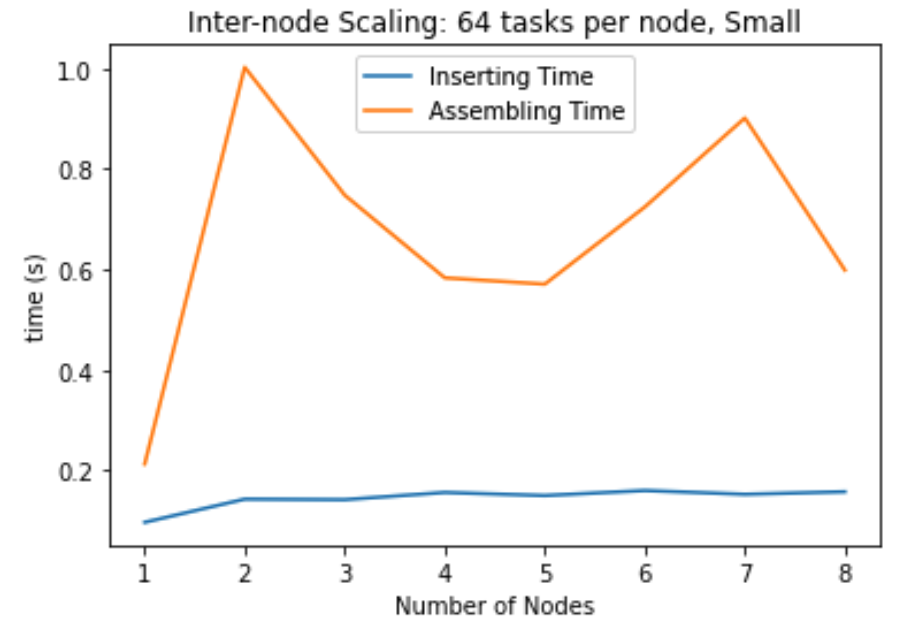
\includegraphics[width=3in]{figures/inter-small-prof.png}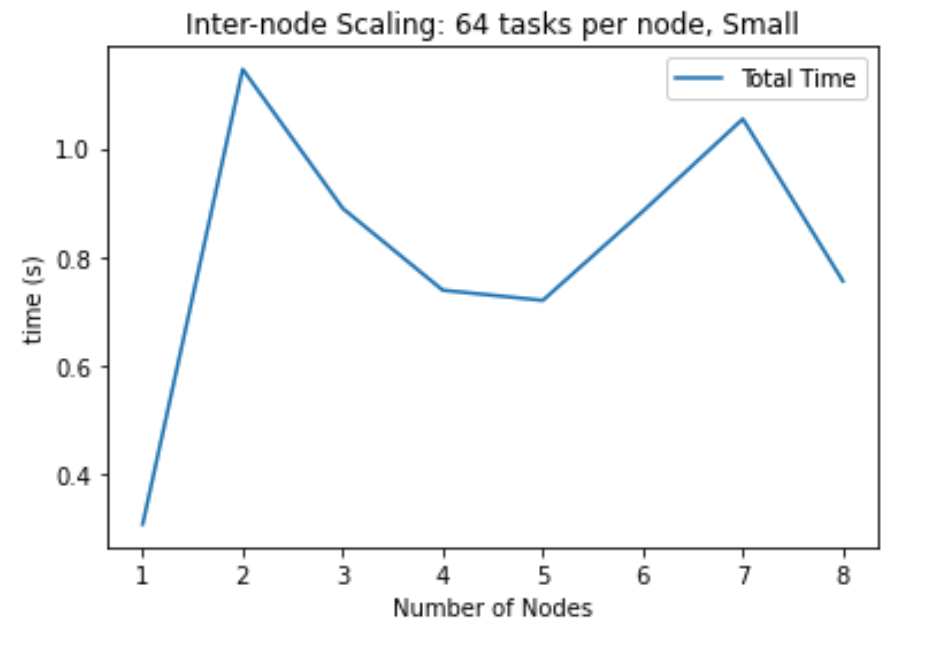
\includegraphics[width=3in]{figures/inter-small.png}}
\subsubsection{Human Synthetic Dataset}
\centerline{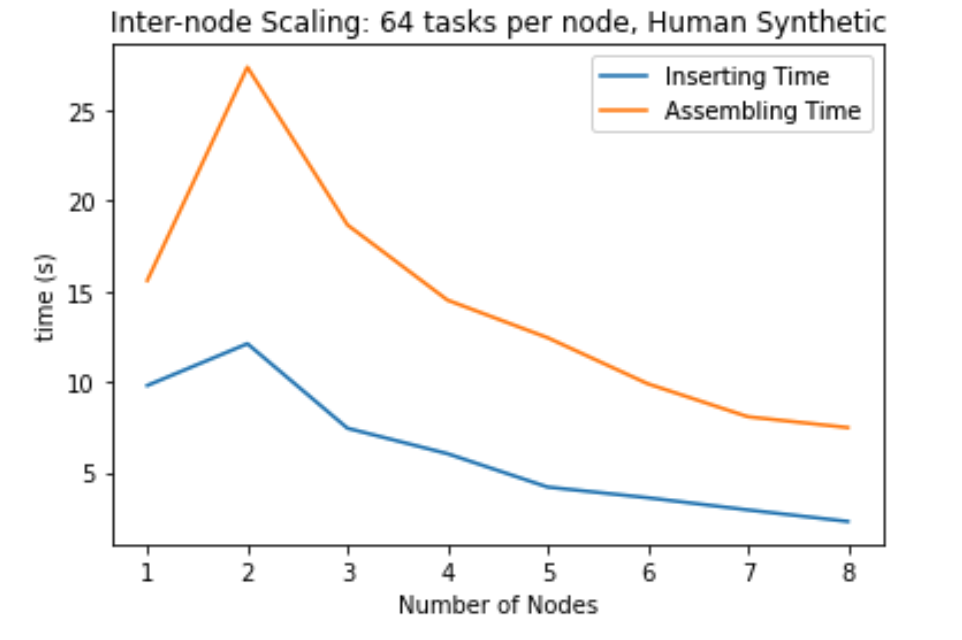
\includegraphics[width=3in]{figures/inter-human-prof.png}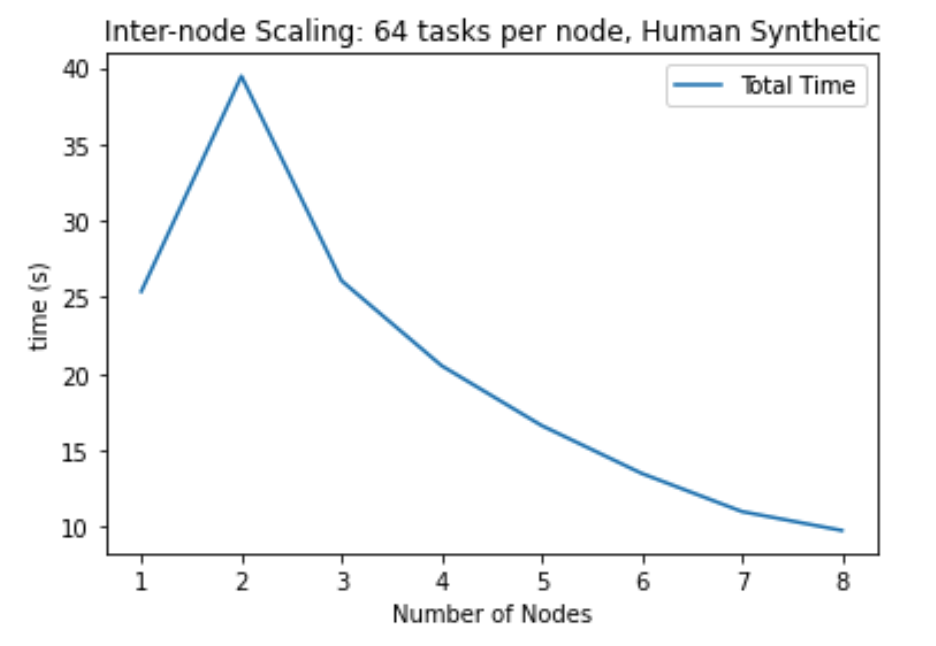
\includegraphics[width=3in]{figures/inter-human.png}}
\subsection{Intra-Node Performance}
\subsubsection{Small Dataset}
\centerline{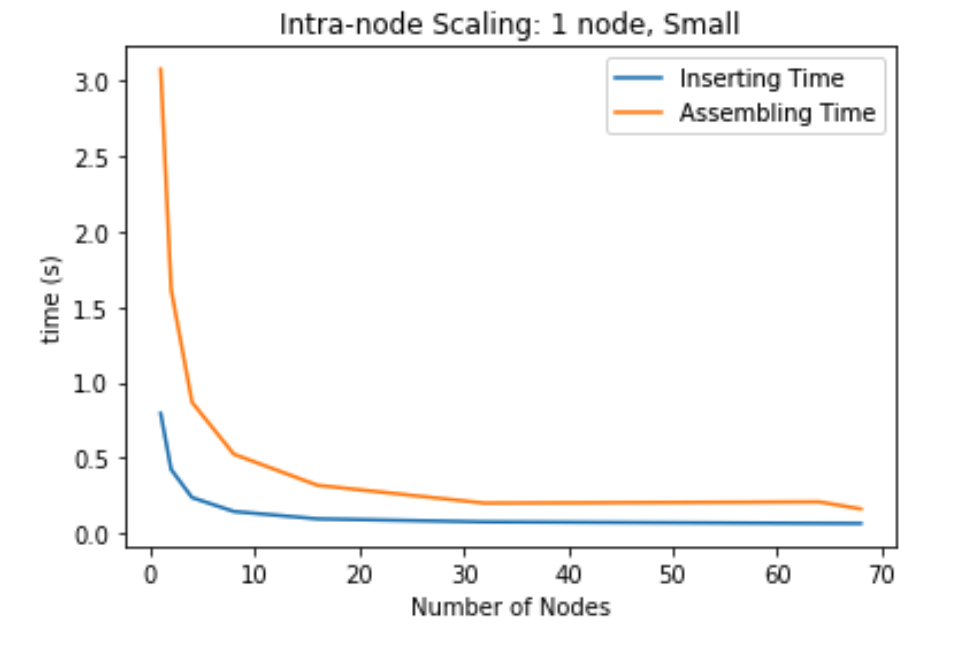
\includegraphics[width=3in]{figures/intra-small-prof.png}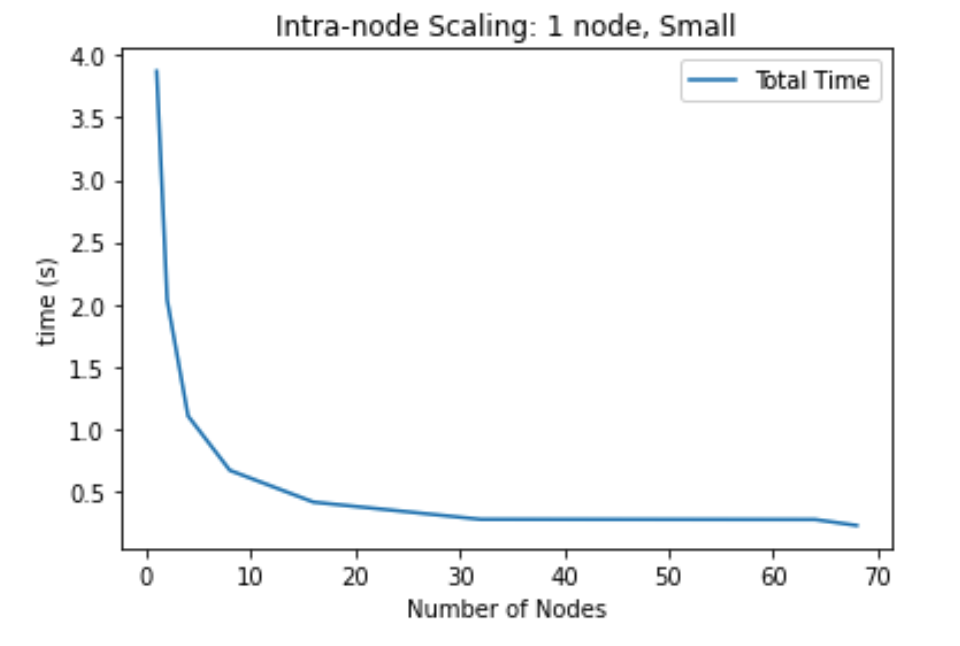
\includegraphics[width=3in]{figures/intra-small.png}}
\subsubsection{Human Synthetic Dataset}
\centerline{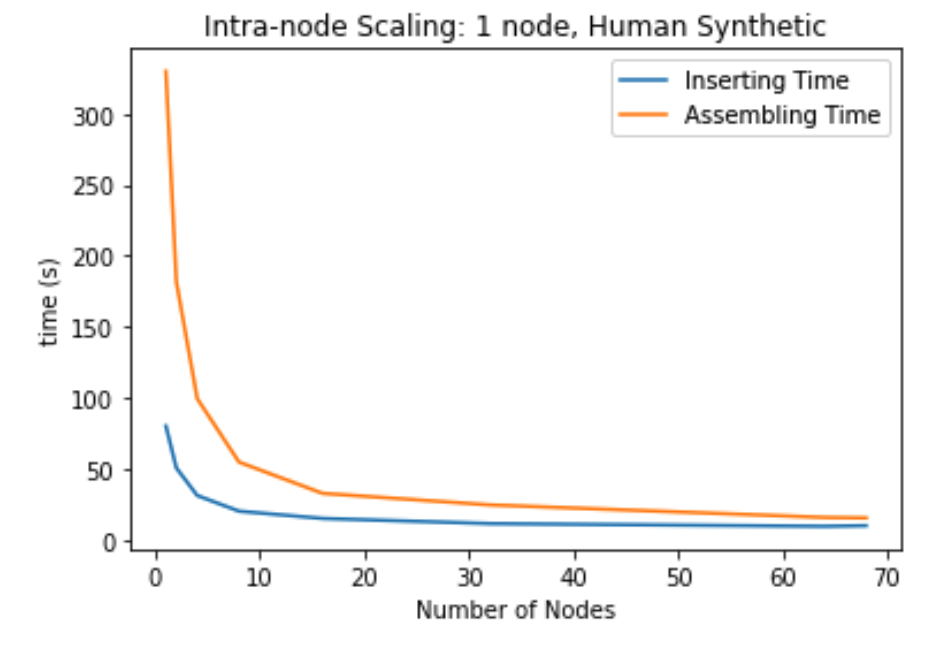
\includegraphics[width=3in]{figures/intra-human-prof.png}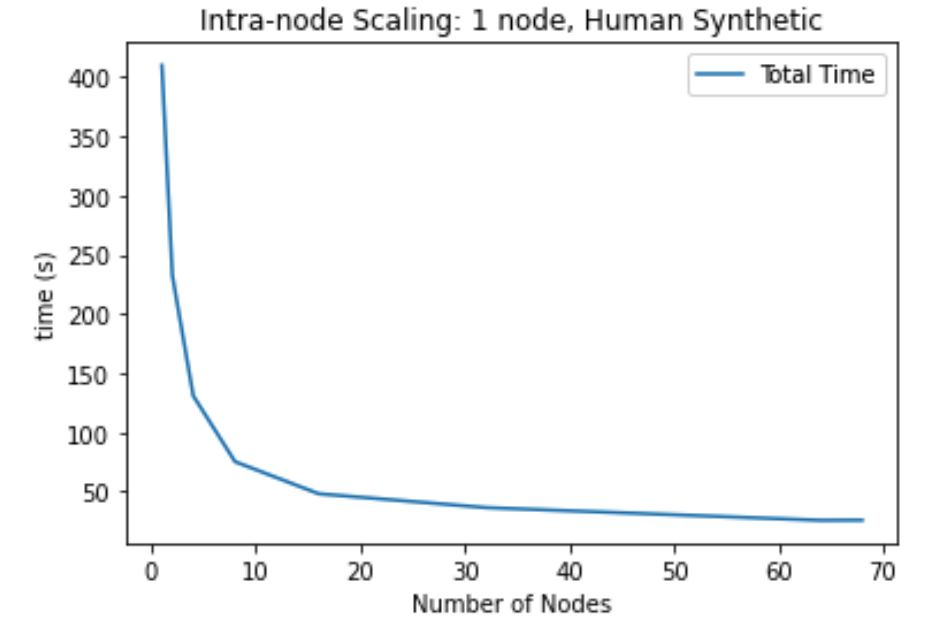
\includegraphics[width=3in]{figures/intra-human.png}}


\subsection{Performance Breakdown}
The human synthetic benchmarks show good scaling with inter-node and intra-node performance. We notice that the curve jumps up sharply and then decreases logarithmically. We suspect the sharp jump in execution time to be the communication overhead when we use multiple nodes. Intra-node performance shows a much steeper and smoother logarithmic code. There is no communication overhead here as it’s all done in shared memory. For smaller datasets, this effect is also replicated, except for the inter-node performance. We think that this is just variance of the benchmark as the difference in time is around 1 second. It appears that the communication overhead on performance of such a small dataset becomes apparent, as 1 node is the only one that performed the best. In general, it seems like our distributed hash table performance scales well, at least for larger datasets!

\section{Contribution}
Kunal, Brian, and Parth all equally worked on all parts of the project.

\bibliographystyle{ieeetr}
\bibliography{references}

\end{document}
